% !TEX program = xelatex
% 공통수학2 · Ⅲ. 함수와 그래프 · 2. 유리함수와 무리함수 · 02 무리함수 · 1/1차시
% 학생용 활동지 (답안 없음)
\documentclass[11pt,a4paper]{article}
\usepackage{kotex}
\usepackage{iftex}
\ifPDFTeX\else
  \setmainhangulfont{Noto Serif CJK KR}
  \setsanshangulfont{Noto Sans CJK KR}
\fi
\usepackage[margin=2.1cm]{geometry}
\usepackage{parskip}
\usepackage{enumitem}
\usepackage{array}
\usepackage{tabularx}
\usepackage{xcolor}
\usepackage{amssymb}
\usepackage{tikz}
\usepackage[most]{tcolorbox}
\usepackage{fancyhdr}
\usepackage{titlesec}

\definecolor{goldc}{HTML}{B07C22}
\definecolor{goldstrong}{HTML}{8A5F16}
\definecolor{indigoc}{HTML}{2B3B57}
\definecolor{indigosoft}{HTML}{6E82A6}
\definecolor{linec}{HTML}{D6DACB}
\definecolor{surface2}{HTML}{E4E8DC}
\definecolor{writeline}{HTML}{C7CCBA}
\definecolor{inksoft}{HTML}{52604F}

\titleformat{\section}{\normalfont\sffamily\bfseries\large\color{indigoc}}{\thesection}{0.6em}{}
\titlespacing{\section}{0pt}{14pt}{6pt}
\newtcolorbox{goalbox}{enhanced, breakable, colback=white, colframe=goldc, boxrule=0.5pt, leftrule=3pt, arc=2pt, left=10pt, right=10pt, top=8pt, bottom=8pt}
\newtcolorbox{sheetbox}{enhanced, breakable, colback=white, colframe=linec, boxrule=0.6pt, arc=3pt, left=11pt, right=11pt, top=9pt, bottom=9pt}
\newcommand{\writespace}[1]{%
  \par\nobreak\vspace{3pt}
  \foreach \n in {1,...,#1} {%
    \noindent\textcolor{writeline}{\rule{\linewidth}{0.4pt}}\par\vspace{0.62cm}%
  }
}
\newcommand{\fillblank}[1]{\makebox[#1]{\hrulefill}}
\pagestyle{fancy}\fancyhf{}\renewcommand{\headrulewidth}{0pt}
\fancyfoot[L]{\footnotesize\color{inksoft} 공통수학2 · 2026학년도 2학기 · 지평선고등학교}
\fancyfoot[R]{\footnotesize\color{inksoft} 다음 시간 --- 중단원·대단원 마무리}

\newcommand{\blankgrid}{%
  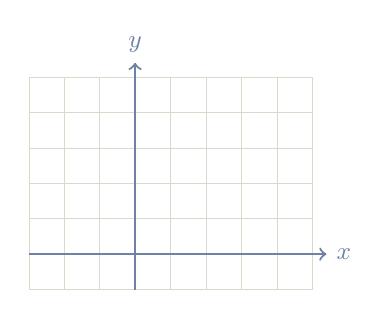
\begin{tikzpicture}[scale=0.45]
    \draw[step=1cm, linec, very thin] (-3,-1) grid (5,5);
    \draw[->, thick, indigosoft] (-3,0) -- (5.4,0) node[right,font=\small]{$x$};
    \draw[->, thick, indigosoft] (0,-1) -- (0,5.4) node[above,font=\small]{$y$};
  \end{tikzpicture}}

\begin{document}

\noindent
\begin{minipage}[b]{0.62\linewidth}
  {\sffamily\footnotesize\color{indigosoft} 공통수학2 · Ⅲ. 함수와 그래프 · 2. 유리함수와 무리함수}\\[2pt]
  {\sffamily\bfseries\Large 02 무리함수 \textperiodcentered\ 41차시}
\end{minipage}\hfill
\begin{minipage}[b]{0.36\linewidth}
  \raggedleft\small\color{inksoft}
  반\ \fillblank{1.6cm} \quad 번호\ \fillblank{1.6cm}\\[4pt]
  이름\ \fillblank{3.6cm}
\end{minipage}

\vspace{4pt}
\noindent{\color{goldc}\rule{\linewidth}{2.2pt}}
\vspace{10pt}

\begin{goalbox}
\textbf{오늘의 목표}\\
무리함수의 뜻을 알고 정의역을 구하며, $y=\sqrt{a(x-p)}+q$의 그래프를 그리고 정의역·치역을 구할 수 있다.
\vspace{4pt}
\small\color{inksoft}
$\square$ 자신 있음 \quad $\square$ 조금 헷갈림 \quad $\square$ 처음 봄 \hfill (수업 전 나의 상태에 표시)
\end{goalbox}

\section{생각 열기 --- 넓이로부터 변의 길이}

\begin{sheetbox}
넓이가 $A$인 정사각형의 한 변의 길이는 $x=\sqrt A$이다. 아래 표를 완성해 보자.

\vspace{6pt}
\begin{tabularx}{\linewidth}{@{}XXXXX@{}}
\toprule
$A$ & $9$ & $4$ & $1$ & $-4$ \\
\midrule
$x=\sqrt A$ & \fillblank{1.6cm} & \fillblank{1.6cm} & \fillblank{1.6cm} & \fillblank{1.6cm} \\
\bottomrule
\end{tabularx}

\vspace{6pt}
$A<0$일 때 $x=\sqrt A$를 구할 수 없는 이유를 한 문장으로 써 보자.
\writespace{2}
\end{sheetbox}

\section{개념 정리 --- 무리함수의 뜻과 정의역}

\begin{sheetbox}
근호 안에 문자를 포함하고, 그 문자가 근호 밖으로 나올 수 없는 식을 \fillblank{2.2cm}이라 하고, 무리식으로 나타낸 함수를 \fillblank{2.4cm}라 한다.

\vspace{6pt}
무리함수 $y=\sqrt{f(x)}$의 정의역은 $f(x)\fillblank{1.4cm}$인 실수 $x$ 전체의 집합이다.

\vspace{8pt}
\textbf{그래프} --- $y=\sqrt{ax}$의 그래프는 $a>0$이면 정의역 $x\fillblank{1cm}0$에서 \fillblank{1.4cm}(증가/감소)하고, $a<0$이면 정의역 $x\fillblank{1cm}0$에서 \fillblank{1.4cm}(증가/감소)한다.

\vspace{6pt}
$y=\sqrt{a(x-p)}+q$의 그래프는 $y=\sqrt{ax}$의 그래프를 $x$축 방향으로 \fillblank{1.4cm}, $y$축 방향으로 \fillblank{1.4cm}만큼 평행이동한 것이다.

\vspace{8pt}
\textbf{예제} --- $y=\sqrt{-x+3}+1$의 정의역과 치역을 구해 보자. 시작점을 먼저 찍고 그래프를 그린다.

\vspace{4pt}
\centering \blankgrid
\end{sheetbox}

\section{연습 문제}

\begin{sheetbox}
\raggedright
\textbf{1.} 다음 중 무리함수인 것을 모두 고르시오.\\
\hspace*{1.6em}① $y=\sqrt{3x-1}$ \quad ② $y=x^2+1$ \quad ③ $y=\sqrt{x+2}-1$ \quad ④ $y=2x-5$
\writespace{2}

\vspace{4pt}
\textbf{2.} $y=\sqrt{2x-4}$의 정의역을 구하시오.
\writespace{2}

\vspace{4pt}
\textbf{3.} $y=\sqrt{-x+3}+1$의 정의역과 치역을 구하고, 그래프가 뻗어나가는 방향을 설명하시오.
\writespace{4}

\vspace{4pt}
\textbf{4.} 정의역이 $\{x\mid x\geq2\}$, 치역이 $\{y\mid y\geq-1\}$이고 점 $(3,1)$을 지나는 무리함수를 $y=\sqrt{a(x-2)}-1$ 꼴로 놓고 식을 구하시오.
\writespace{3}
\end{sheetbox}

\section{사고의 가시화 --- See · Think · Wonder}

\noindent{\footnotesize\color{inksoft} 오늘 배운 `무리함수'를 떠올리며 아래 세 칸을 채워 보자.}\\[6pt]
\begin{tabularx}{\linewidth}{@{}XXX@{}}
\textbf{\footnotesize\color{indigoc} See --- 무엇을 보았나?} &
\textbf{\footnotesize\color{indigoc} Think --- 무엇을 생각했나?} &
\textbf{\footnotesize\color{indigoc} Wonder --- 무엇이 궁금한가?} \\[4pt]
\end{tabularx}
\noindent
\begin{minipage}[t]{0.32\linewidth}\writespace{3}\end{minipage}\hfill
\begin{minipage}[t]{0.32\linewidth}\writespace{3}\end{minipage}\hfill
\begin{minipage}[t]{0.32\linewidth}\writespace{3}\end{minipage}

\section{마무리 성찰}

\begin{sheetbox}
\begin{minipage}[t]{0.48\linewidth}
{\footnotesize\color{inksoft} 무리함수의 정의역을 구하는 방법을 한 문장으로}
\writespace{2}
\end{minipage}\hfill
\begin{minipage}[t]{0.48\linewidth}
{\footnotesize\color{inksoft} 감사 일기 / 유념 한 줄}
\writespace{2}
\end{minipage}
\end{sheetbox}

\end{document}
